%!TEX root =../cmbs4_scibook.tex
%%%%%% CMB-S4 DE/DM Chapter  %%%%%%%%%%%%%%%%

\chapter{Dark Energy and Dark Matter}

\section{Dark Energy and Modified Gravity}

\subsection{Introduction}

The enigma of cosmic acceleration is among the most challenging problems in physics. Our most basic understanding about gravity -- that objects fall towards one and other under mutual gravitational attraction -- simply does not apply on the largest distance scales. Instead, gravity is apparently repulsive at large distances and late times; the scale of spacetime itself is currently not only expanding but accelerating. The implication is either that our understanding of gravity is incomplete, or some other causative agent -- dark energy -- with exotic gravitational properties fills the universe. In both cases, new physics is required beyond the four fundamental forces described by the Standard Model and general relativity.

The working hypothesis is that the cosmic acceleration is due to an exquisitely small cosmological constant, that Einstein's general relativity is valid from millimeter to beyond gigaparsec scales, and that dark matter consists of a single species of a cold, collisionless particle. Yet none of these offer insight or reflect the unity of physics demonstrated elsewhere as in the Standard Model of particle physics.

In particular, the cosmological constant suffers from a naturalness problem whose resolution may lie in a dynamical dark energy, quintessence. Theories of quintessence posit a new scalar field and predict a variety of testable phenomena.  They can also unveil new links to dark matter, neutrino physics, and cosmic parity violation. In their most general form, they represent
a scalar-tensor theory of gravity which can be described by  the effective field theory (EFT) of cosmic acceleration in the linear regime. 
CMB-S4 can provide the hard evidence  needed to pare down these possibilities and potentially discover clues to the enigma of cosmic acceleration that will enable the development of  compelling theoretical 
alternatives to the cosmological constant.

% possibly redundant... eventually streamline.
In summary, the current observational evidence suggests a new frontier for physics at low energies and weak coupling, implied by the cosmological scales that characterize cosmic acceleration.CMB lensing, thermal SZ cluster counts and mass measurements, and the kinematic SZ effect  all measure the influence of cosmic acceleration on the growth of 
structure.   As such, CMB-S4 would be capable of helping to answer basic questions about dark energy and gravity in a manner complementary to ongoing precision measurements of the expansion history.    % and dark matter (restore later if we merge).


\subsection{Models and parameters}


In this section, we  briefly review the models and frameworks that have been proposed over the past years to test dark energy and modified gravity.   These fall into 
three families: ``trigger'', equations of motion, and theory parametrizations. The first ones are aimed at testing and falsifying the standard model
of $\Lambda$CDM, a cosmological constant with cold dark matter, and are agnostic as to its 
alternatives.  Given precise measurements from primary CMB anisotropy of the high redshift universe, all low redshift observables related to the expansion history and growth of
structure are potential triggers.  Trigger parameters thus have the benefit that their relationship to the raw observables can be made as direct as desired.   The drawback is 
that deviant values for the trigger may not have any physical motivation.  Instead they help pare down the possibilities for the more model
dependent and theory oriented tests.  


  In the next section we discuss the cluster abundance,
 CMB lensing and pairwise kinematic SZ effects as the building blocks of triggers when
 combined with other measurements such as BAO and SNIa.   CMB-S4 will also enhance the precision and robustness
 of these other tests by measurements of the primary $E$-mode polarization.   For example
 the cold dark matter $\Omega_c h^2$ and effective relativistic degrees of freedom $N_{\rm eff}$ enter into the calibration of the BAO scale as well as inferences on $H_0$. 
 
In addition to triggers based on the expansion history, CMB-S4 provides triggers based
on the growth of structure.  The $\Lambda$CDM model predicts that the growth of structure
will slow in a precisely known manner as the expansion starts to accelerate.   
For example the rms amplitude of linear matter fluctuations at the $8 h^{-1}$Mpc
scale $\sigma_8(z)$ is a trigger parameter that can be closely associated with the 
cluster abundance.   The linear growth rate index $\gamma$ is another that is closely related
to peculiar velocities and the kSZ observables.   
% add in $E_G$ if we forecast it or if it is discussed in the cross correlation section.

The second way of parametrizing deviations from $\Lambda$CDM is by modifying the equations of motion for dark energy in a manner consistent with conservation laws.   These have the benefit of attempting to tie distance and growth
tests together in a physical, yet still phenomenological manner.    The next step up in
complexity from a cosmological constant is a model where the dark energy is dynamical
but spatially smooth relative to the dark matter.   In these models, the expansion history
can deviate from that of $\Lambda$CDM due to evolution in  the dark energy
equation of state $w(z)$, yet still predict the growth of structure.   A common parameterization
of this phenomenology is
\begin{equation}
w(z) = w_0 + w_a \frac{z}{1+z}.
\end{equation}
The figure of merit defined by the DETF is the inverse area of the
95\% CL region in the $w_0-w_a$ plane.  

There are generalizations of this type of parameterization that separate the expansion history from 
the growth of structure.   
A complete parametrization for observables for scalar-tensor theories in the linear regime would include in addition
the gravitational slip or effective anisotropic stress  (the ratio of the space curvature potential and Newtonian potential),  the effective Newton constant, and  $c_T$ the
speed of tensor perturbations. [intentionally vague on which notation to use: forecaster will
decide the favorite one and supply details.  Possibly add graviton mass as it is mentioned
in Inflation chapter.]

%
The last way of studying deviations from $\Lambda$CDM consists in directly testing theories beyond it.  Given the lack of a compelling specific theory to test, we can still make progress
by parameterizing all possible Lagrangians for fluctuations that are consistent with the
given symmetry.
 This approach maintains a strong connection with the underlying theory at the price of
complicating the relation to the raw data.  

More specifically, a systematic implementation of this approach is the effective field theory (EFT)
of cosmic acceleration \cite{Gubitosi:2012hu,Bloomfield:2012ff}, inspired by the EFT  of inflation described in the Inflation Chapter~\cite{Creminelli:2006xe,Cheung:2007st,Weinberg:2008hq,Creminelli:2008wc,Park:2010cw,Jimenez:2011nn}.    The EFT of cosmic acceleration describes the cosmological phenomenology of all universally coupled single scalar field dark energy and modified gravity models. Specifically, the EFT action is constructed in a unitary gauge to preserve isotropy and homogeneity of the cosmological background and reads:
%
\begin{eqnarray} \label{Eq:EFTaction}
\mathcal{S}_{\rm EFT} = \int d^4x \sqrt{-g}&& \bigg\{ \frac{m_0^2}{2} \left[1+\Omega(\tau)\right] R + \Lambda(\tau) - c(\tau)\,a^2\delta g^{00} + \frac{M_2^4 (\tau)}{2} \left( a^2\delta g^{00} \right)^2 \nonumber \\ 
&&   - \frac{\bar{M}_1^3 (\tau)}{2} \, a^2\delta g^{00}\,\delta K{^\mu_{\,\,\mu}}  - \frac{\bar{M}_2^2 (\tau)}{2} \left( \delta {K}{^\mu_{\,\,\mu}}\right)^2   - \frac{\bar{M}_3^2 (\tau)}{2} \,\delta {K}{^\mu_{\,\,\nu}}\,\delta {K}{^\nu_{\,\,\mu}} \nonumber \\
&& + m_2^2(\tau)\left(g^{\mu\nu}+n^{\mu} n^{\nu}\right)\partial_{\mu}(a^2g^{00})\partial_{\nu}(a^2g^{00}) +\frac{\hat{M}^2(\tau)}{2} \, a^2 \delta g^{00}\,\delta \mathcal{R}+	\ldots \bigg\}  \nonumber \\
&& + S_{m} [g_{\mu \nu}, \chi_m ]
\end{eqnarray}
%
where $R$ is the four-dimensional Ricci scalar, $\delta g^{00}$, $\delta K{^\mu_{\,\,\nu}}$, $\delta K{^\mu_{\,\,\mu}}$ and  $\delta \mathcal{R}$ are, respectively, the perturbations of the upper time-time component of the metric, the extrinsic curvature and its trace and the three dimensional spatial Ricci scalar of constant-time hypersurfaces. Finally,  $S_m$ denotes the action for all the matter fields conventionally considered in cosmology. 

In the action (\ref{Eq:EFTaction}), the  extra scalar degree of freedom is hidden inside metric perturbations. 
To study the dynamics of linear perturbations, however, it is convenient to make it explicit by means of  the St\"{u}ckelberg technique i.e.~performing an infinitesimal coordinate transformation such that $\tau\rightarrow \tau+\pi$, where the field $\pi$ describes the extra propagating degree of freedom. This approach allows us to maintain a direct link to the underlying theory so that we can keep under control its theoretical viability while exploring the cosmological implications of any of the models included in this language~\cite{Raveri:2014cka}. 

Since the choice of the unitary gauge breaks time diffeomorphism invariance, each operator allowed by the residual symmetry, in action (\ref{Eq:EFTaction}), can be multiplied by a time-dependent coefficient that we shall call EFT function. To fully specify the phenomenology of linear perturbations only a restricted set of EFT functions are needed. These can be either parametrized to explore agnostically the space of dark energy and modified gravity models~\cite{Gleyzes:2013ooa,Bloomfield:2013efa,Piazza:2013coa,Gleyzes:2014rba} or can be fixed to reproduce exactly the phenomenology of some model of interest such as $f(R)$ gravity, quintessence and, more generally, the Horndeski class of theories and beyond~\cite{Gleyzes:2014dya,Frusciante:2015maa,Frusciante:2016xoj}.
%
\subsection{CMB  Dark Energy Observables}

\subsubsection{Cluster abundance and mass}

Clusters of galaxies are sensitive to the content, geometry, and growth of structure in the universe.     In the report of the DETF, they were highlighted as having the highest sensitivity
to dark energy parameters  but simultaneously the largest astrophysical systematic due
to uncertainties in the mass scaling of the cluster observables.   In the ``Stage IV" era of
dark energy probes, CMB-S4 will play a critical role in overcoming this challenge.




Clusters of galaxies are the most massive ($\sim$10$^{14}$-10$^{15}$ M$_{\odot}$) objects in the universe to have underwent gravitational collapse, 
having formed from regions $\sim$10-40 Mpc.  This property makes clusters representative of the overall content of the universe, and also makes them 
important tracers of the evolution of large-scale structure, sampling the most extreme peaks in the large-scale matter distribution.  
These properties have enabled clusters to make important contributions to cosmology: the discovery of dark matter in the 
Coma cluster \cite{1933AcHPh...6..110Z}, 
providing early evidence for $\Omega_m < 1$ \cite{white93a, Donahue98, Bahcall98}, and
constraining the physical nature of dark matter \cite{Clowe06}.  
More recently, measurements of clusters have been used to constrain the properties of dark energy and modifications 
to gravity \cite{vikhlinin09, mantz10a, rapetti13, benson13, mantz14, mantz15}.   In the future era of ``Stage IV'' dark energy 
facilities such as DESI and LSST, measurements of the abundance of galaxy clusters can make complementary and 
competitive constraints on the dark energy equation of state and deviations from General Relativity \cite{weinberg13}.  

CMB measurements find clusters through the inverse Compton scattering of CMB photons off of intra-cluster gas, otherwise 
known as the Sunyaev-Zel'dovich (SZ) effect \cite{sunyaev72}. SZ cluster surveys have two important advantages: 
the SZ surface brightness is redshift independent, and the integrated SZ signal is expected to be a relatively 
low-scatter cluster observable \cite{nagai06, nagai07, kravtsov12}.  These properties enable SZ surveys to provide 
relatively clean, mass-limited cluster catalogs out to high-redshift ($z > 1$).  Since the first SZ-discovered clusters were 
report in 2009 \cite{staniszewski09}, SZ surveys have produced catalogs of over 1000 SZ-selected clusters extending out to $z \sim 1.7$ 
\cite{vanderlinde10, reichardt13, hasselfield13, planck13-29, bleem15b, planck15-32}.  


Figure \ref{fig:limits} shows an estimate of the mass sensitivity, expressed as the one-sigma mass uncertainty as a function of redshift, for two possible CMB-S4 configurations and compares them to planned CMB experiments. 
In Figure \ref{fig:cluster_counts}, we show projections for the mass-threshold and total cluster counts for three possible CMB-S4 configurations.  
The 50\% mass-completeness threshold for the CMB-S4 cluster survey would be relatively flat with redshift out to $z \sim 2$.  
The mass-threshold increases from $\sim$1-2 $\times$ 10$^{14}$ M$_{\odot}$, going from a CMB-S4 angular resolution 
of 1 to 3 arc-minutes, which is $>$2 times lower than current SZ surveys even in the worse case scenario for CMB-S4.  
In addition, the lower mass threshold and larger sky area of CMB-S4, would translate to a nearly $\sim$100 fold increase in the 
number of SZ-identified clusters.  At a 99\% purity threshold, for a configuration with a 1, 2, and arc-minute angular 
resolution, CMB-S4 would identify $\sim$40,000, 70,000, and 140,000 clusters, respectively.  


\begin{figure}[t]
\begin{center}
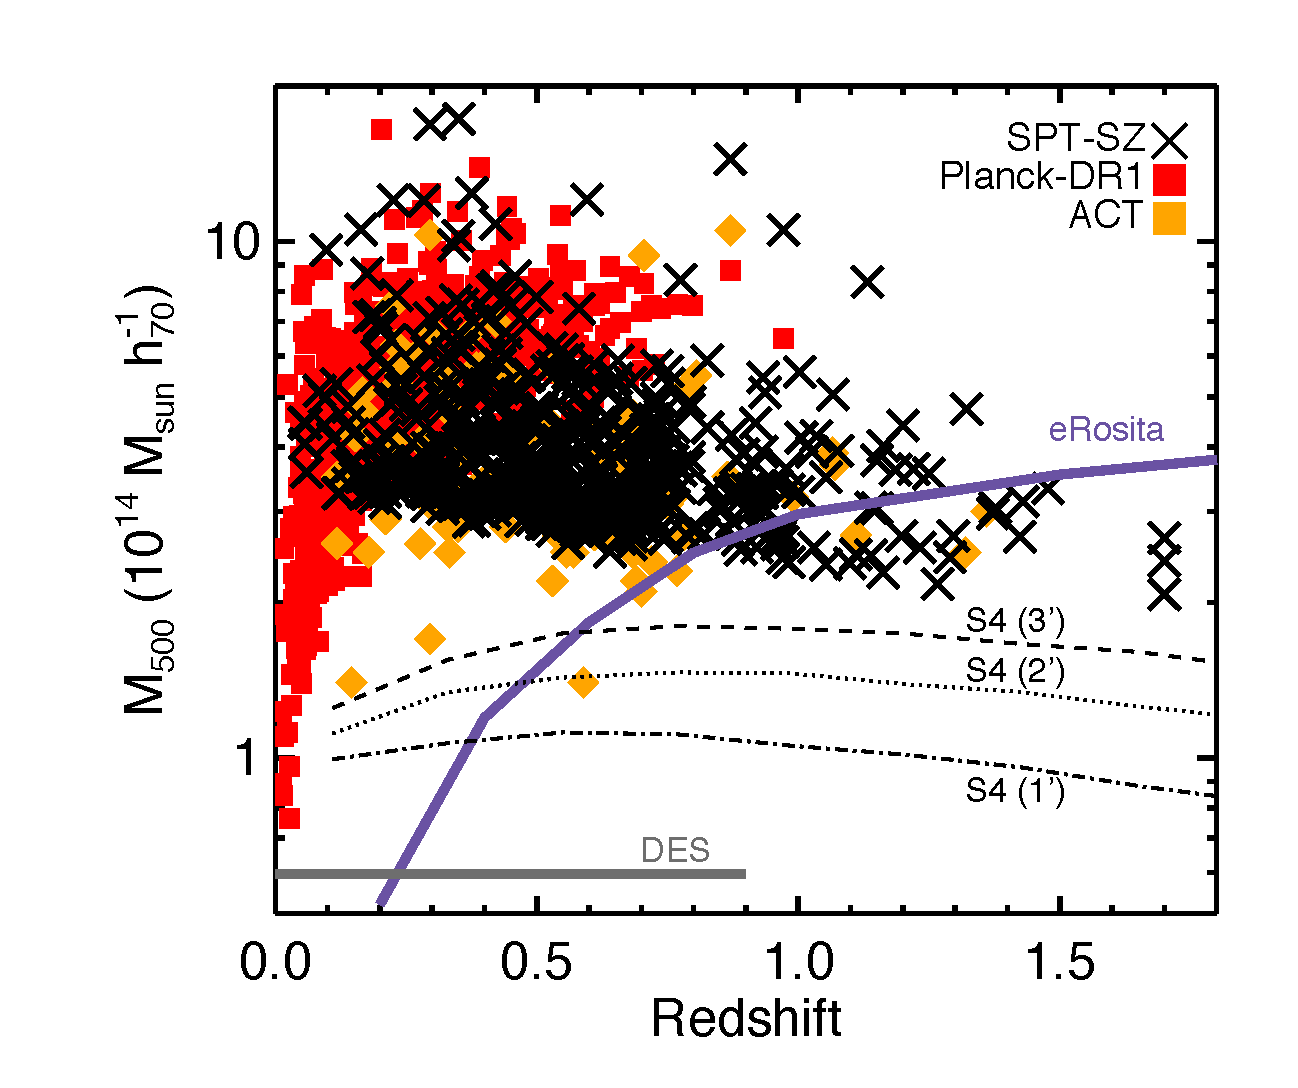
\includegraphics[width=0.49\textwidth]{DarkEnergy/mass_vs_z_s4.pdf}
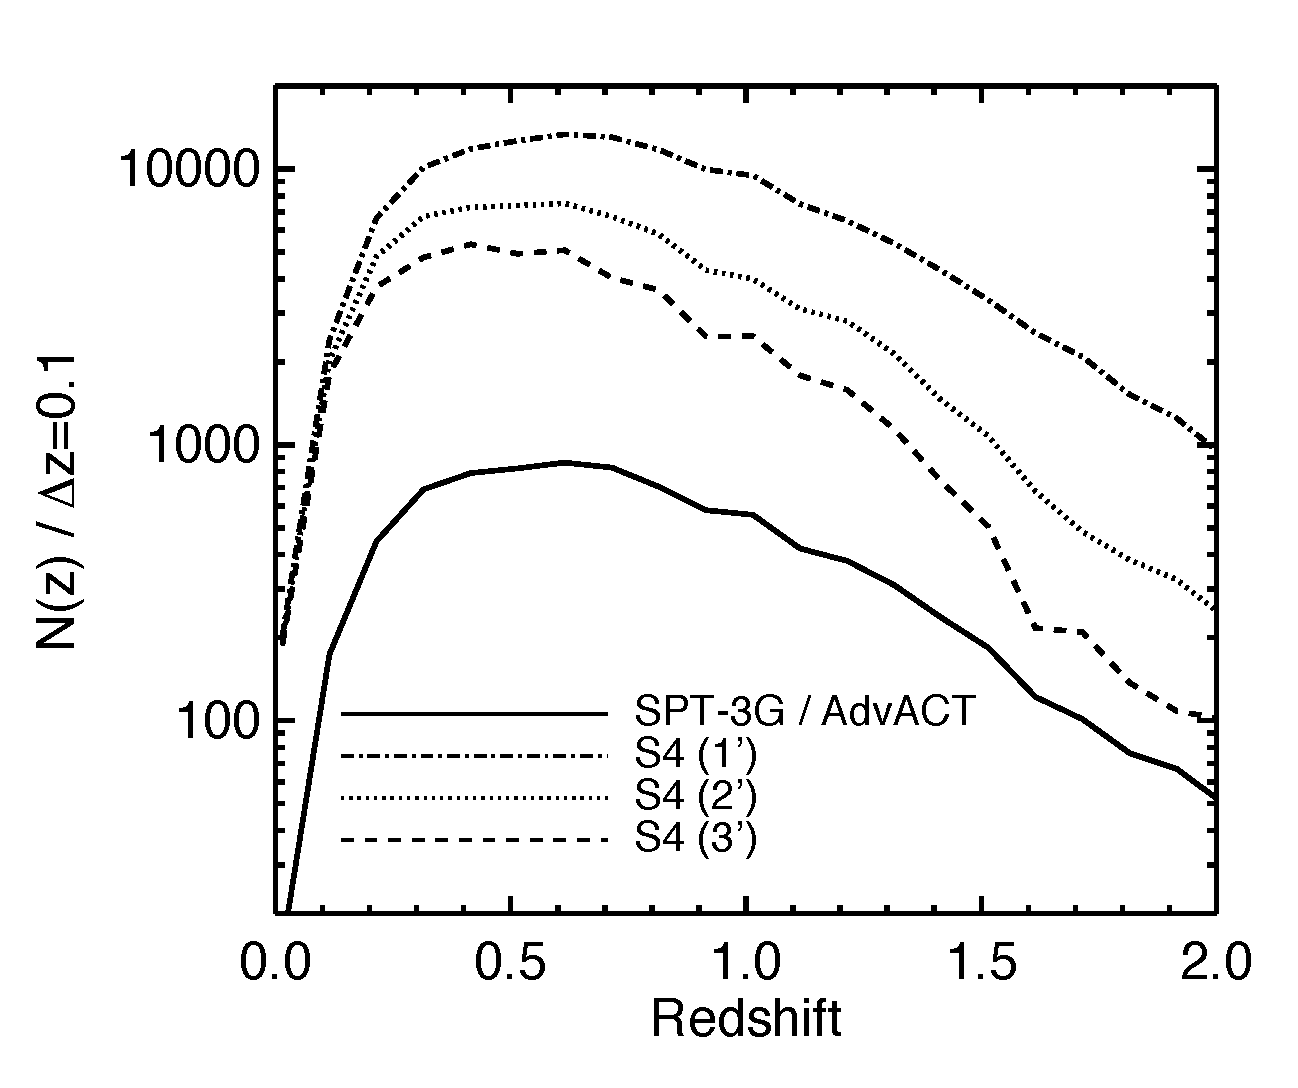
\includegraphics[width=0.49\textwidth]{DarkEnergy/dndz_s4.pdf}
\caption{(Left) The 50\% mass-completeness limits for three possible CMB-S4 instrumental configurations with either 1, 2, or 3 arc minute angular resolution.  For comparison, this can be compared with existing SZ-selected cluster catalogs from Planck \cite{planck15-32}, SPT-SZ \cite{bleem15b}, and ACT \cite{hasselfield13}, and future thresholds expected for the optical Dark Energy Survey and the X-ray eRosita survey \cite{pillepich12}.  (Right) The projected cluster counts for the three possible CMB-S4 configurations described above.  For comparison, the projected cluster counts from the SPT-3G \cite{benson14} and AdvACT surveys.}
\label{fig:cluster_counts}
\end{center}
\end{figure} 

CMB-S4 will also enable a new means of calibrating cluster masses through CMB lensing.
Accurate masses are crucial for catalogs to provide constraints on dark energy and modified gravity.
With sufficient angular resolution, CMB-S4 opens tremendous possibilities for measuring cluster, more generally halo masses.    
  Figure \ref{fig:limits} shows an estimate of the mass sensitivity, expressed as the one-sigma mass uncertainty as a function of redshift, for two possible CMB-S4 configurations and compares them to planned CMB experiments. 


	The estimation is made assuming foreground subtraction to reach the quoted CMB map noise level at the given angular resolution.  The method (Melin \& Bartlett 2015) employs an optimal filter matched to the NFW profile and applied to reconstructions of the lensing potential with a quadratic estimator (Hu \& Okamoto 2002).  The method has already been successfully applied to the Planck cluster cosmology sample of more than 400 objects (Planck Collaboration XXIV 2015).  This figure shows the sensitivity obtained with just CMB temperature lensing reconstruction.  Including polarization will significantly improve it.  
	We see that the mass sensitivity remains flat with redshift, a remarkable property that enables mass estimation out to redshifts unreachable with galaxy shear measurements.  This is a powerful and unique capability of CMB lensing.  The figure also demonstrates the important gains attained with high angular resolution.  At one arcmin resolution, S4 achieves a mass sensitivity of $2 \times 10^{13}M_\odot$ with temperature alone.  This unprecedented sensitivity not only ensures robust mass estimation for cluster cosmology over the large redshift interval where S4 will detect clusters through the SZ effect, but also paves the way to numerous cluster and large-scale structure studies.  The rapidly increasing science reach enabled by high angular resolution, approaching one arcmin, is an important consideration in CMB-S4 objectives.  

\begin{figure}[t!]
\begin{center}
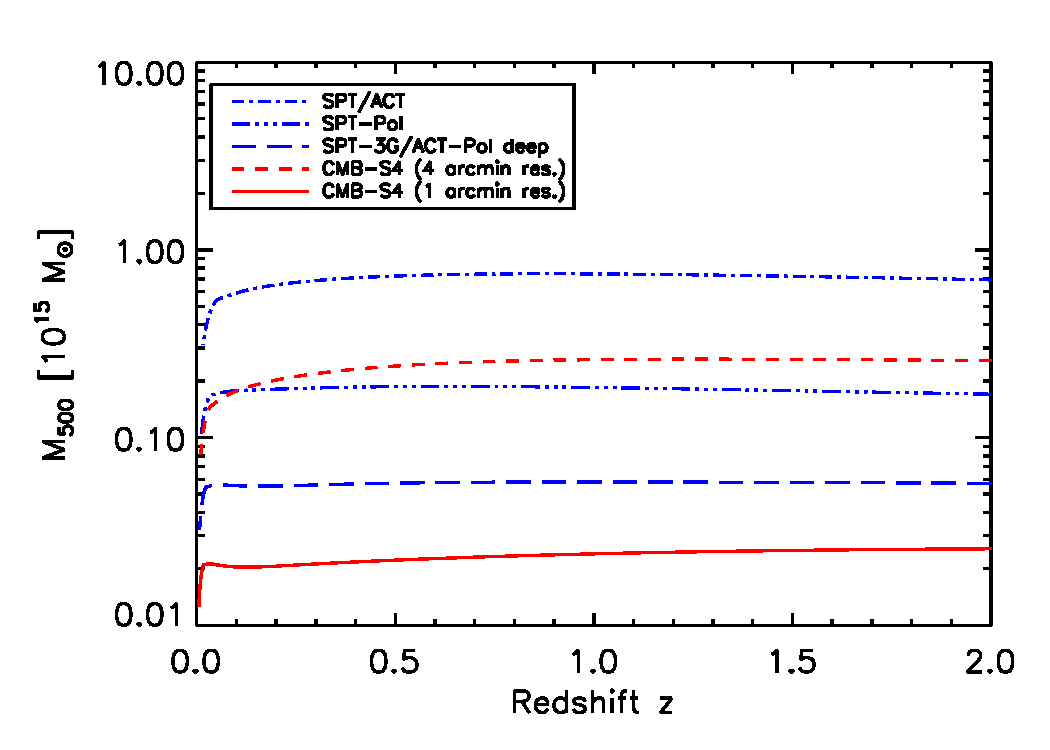
\includegraphics[width=0.65\textwidth]{DarkEnergy/m500lim_vs_z_1sigma_cmbs4_v1.pdf}
\caption{Cluster mass sensitivity of CMB lensing.}
\label{fig:limits}
\end{center}
\end{figure} 

\subsubsection{Lensing}

As described in the Lensing Chapter, the CMB lensing deflection map measures the projected mass density all the way back to the decoupling epoch at $z \sim 1100$, with the majority of the contributions coming from $z > 1$.  CMB lensing is also dominated by structure on large scales in the linear regime.  Thus,  CMB lensing provides a clean probe of a particular integral over the linear growth of structure,
e.g.~$\sigma_8(z)$,
weighted by distances. The lensing power spectrum shape is predicted from the background cosmology; shape deviations indicate scale-dependent effects on the growth, including those caused by modified gravity or the 
gravitational effects of dark energy.  CMB lensing complements other dark energy probes by providing
a handle on effects at high redshift, e.g. in so-called early dark energy scenarios.

Cross-correlating the CMB lensing with other tracers of structure further permits extraction of information about the growth rate of structure in the universe that is localized in redshift.  To the extent that other tracers have well-understood redshift distributions, cross-correlating a set of them to the CMB constitutes a tomographic study probing the evolution of the dark energy and its impact on the growth rate. The Lensing Chapter catalogs two broad categories of other tracers: galaxy density fields (and by extension the CIB) and galaxy shear maps. Combining lensing maps with maps of large scale flows from the kSZ will provide further constraints on the dark energy.

Another key contribution from CMB lensing to the study of dark energy will be its complementarity to other Stage IV experiments, including DESI and LSST, as well as EUCLID and WFIRST. (CMB Lensing chapter already mentions forecasting the improvement on calibrating multiplicative bias for LSST Ð would it make sense to move that here?) Not only will CMB lensing provide a new redshift kernel for tomography studies, it will also validate or improve the calibration for LSST, increasing its DE FOM by a factor of xxx.

%To include: forecasts for wa vs w0 (or whatever final parameterization is desired) for BOSS, then BOSS + CMB S4; for DESI+BOSS, then add in CMB S4; etc. 



\subsubsection{Kinematic SZ}

% Edited by F. de Bernardis
CMB-S4 will map with unprecedented precision the momentum field of the large scale structure via measurements of the kinematic Sunyaev Zel'dovich (kSZ) effect. Multi-frequency data can be used to remove other foregrounds and isolate the kSZ signal. CMB-S4 measurements with sufficient angular resolution can be used to reconstruct the diffuse kSZ anisotropy signal enabling sub-percent precision measurements of the amplitude of the matter density fluctuations $\sigma_8$ (see for example \cite{Calabrese:2014gwa}) while measurements of the patchy kSZ can place strong constraints on the time and duration of reionization.

The combination of CMB-S4 with data from galaxy surveys will be able to measure the kSZ effect associated with galaxy clusters, which is proportional to their peculiar momentum. The large scale structure momentum field is an important cosmological observable that can place strong constraints on the cosmological parameters \cite{Bhattacharya:2007sk,Kosowsky:2009nc,Mueller:2014nsa,Mueller:2014dba} complementary to density fluctuations field measurements. The mean pairwise velocity of galaxy clusters is sensitive to both the growth of structure and the expansion history of the universe and it is an excellent probe for gravity on large scales. Being a differential measurement it is also particularly stable against residual foregrounds that might survive the frequency cleaning process. In \cite{Mueller:2014nsa,Mueller:2014dba} it has been shown that a S4 survey with high resolution can constrain the redshift dependent growth of structure at $\lesssim 5\%$ precision in generic models allowing also for a redshift dependent equation of state of the dark energy. These measurements will be able to distinguish dark energy from modified gravity and will provide complementary constraints to redshift space distortions and weak lensing measurements, probing larger physical scales.

kSZ pairwise measurements can also constrain the sum of neutrino masses $M_{\nu}= \sum m_{\nu}$ with a $1\sigma$ uncertainty of $0.030$eV for a $1$ arcmin CMB-S4 overlapping 10000 deg$^2$ with a galaxy survey able to identify $M>10^{13}M_{\odot}$ clusters. With a 5 arcmin resolution separating the CMB background from the kSZ signal would be more difficult, providing  $\sigma_{M_{\nu}} = 0.076$eV (de Bernardis et al., in preparation). These forecasts include only priors on the 6 standard cosmological parameters from Planck temperatures data and show the potential of the kSZ pairwise signal to provide constraints on the neutrino mass. 

%
% Forecasts for the final book here or if more appropriate e.g. trigger type then embedded
% in the sections themselves
%
%
%\subsection{Forecasts}
%
%\begin{itemize}
%\item First forecast possible in 1 or 2 weeks timescale on all models in EFTCAMB;
%\item Discuss the observational status of these parametrizations;
%\item Discuss critical/natural threshold;
%\end{itemize}
%



\section{Dark Matter}
%  currently spit off into its own chapter we may remerge them when sections are more complete


We have learned from many different experiments (weak and strong lensing, studies of the Bullet Cluster, the Cosmic Microwave Background, etc) that approximately $84\%$ of all the matter in the universe is composed of dark matter, which is not accounted for by the Standard Model of particles. However, the particle nature of dark matter remains unknown.

There are various types of experiments trying to shed light on this question: direct detection experiments, indirect detection experiments, and collider experiments. 
An alternative observable where Dark Matter interactions can modify the Standard Model prediction is the CMB power spectrum.
CMB-Stage IV will have the sensitivity to detect new cosmological signatures originating from various types of dark matter interaction. In the sections below, we will discuss some of these possible scenarios.

\subsection{Dark Matter Annihilation}

One of the leading candidates for dark matter are the Weakly Interactive Massive Particles (WIMPs). If dark matter consists of WIMPs, we would expect these particles to self-annihilate. The annihilation of dark matter produces a shower of very energetic particles, that injects energy into the universe, ionizing the matter in it.

This extra source of ionization has distinctive effects on the Cosmic Microwave Background (CMB): it suppresses the CMB temperature and polarization fluctuations at small angular scales, and it enhances the CMB polarization fluctuations at large angular scales due to the extra scattering of photons off free electrons \cite{Chen:2003gz,Padmanabhan:2005es}.
CMB temperature and polarization spectra can constrain the parameter
$p_{\rm ann}=f\langle\sigma v\rangle/m_{\rm DM}$, where $f$ is the fraction of energy
deposited into the plasma, $\langle\sigma v\rangle$ is the velocity-weighted
cross section, and $m_{\rm DM}$ is the mass of the DM particle.
Current constraints coming from WMAP 9-year data,
Planck, ACT, SPT, BAO, HST and SN data excluded
Dark Matter masses below $26$ GeV at the 2$\sigma$ level, assuming that
all the energy is deposited in the plasma \cite{Madhavacheril:2013cna}. CMB-Stage IV is expected to tighten these constraints by a factor of $10$ \cite{Wu:2014hta}. Dark-matter annihilation also leads to growing ionization fraction perturbations and amplified small-scale cosmological perturbations, leaving an imprint on the CMB bispectrum \cite{Dvorkin:2013cga}.

%
\subsection{Dark Matter-Dark Radiation Interaction}
%
Near the epoch of CMB last scattering, dark matter accounts for about $65\%$ of the energy budget of the Universe, hence making the CMB a particularly good probe of potential new physics in the dark matter sector. Of particular relevance to CMB-S4 studies, the presence of new dark matter interactions with light degrees of freedom \cite{Goldberg:1986nk,1992ApJ...398...43C,1992ApJ...398..407G,1994ApJ...431...41M,1995ApJ...452..495D,AtrioBarandela:1996ur,Boehm:2001hm,Foot:2004pa,Green:2005fa,Profumo:2006bv,Mangano:2006mp,Ackerman:2008gi,ArkaniHamed:2008qn,Feng:2009mn,Serra:2009uu,Bringmann:2009vf,Kaplan:2009de,McDermott:2010pa,Kaplan:2011yj,Aarssen:2012fx,Diamanti:2012tg,Baldi:2012ua,Cline:2012is,Cyr-Racine:2013ab,Fan:2013yva,Fan:2013tia,Cyr-Racine:2013fsa,Bringmann:2013vra,Wilkinson:2013kia,Dvorkin:2013cea,Boehm:2014vja,Wilkinson:2014ksa,Escudero:2015yka,Chu:2014lja,Archidiacono:2014nda,Buen-Abad:2015ova,Lesgourgues:2015wza} can leave subtle imprints on the temperature and polarization CMB power spectra. The introduction of such non-minimal dark matter models has been primarily (but not exclusively) motivated in the literature by potential shortcomings of the standard cold dark matter scenario at small sub-galactic scales \cite{deBlok:1997zlw,Klypin:1999uc,Moore:1999aa,Zavala:2009ms,Oh:2010ea,BoylanKolchin:2011de,Papastergis:2011xe,Walker:2011zu,Pawlowski01112013,Klypin:2014ira,Oman:2015xda,Papastergis2015de}. While these issues are far from settled, they motivate the search for other non-minimal dark matter signatures in complementary data sets (such as the CMB) that could indicate whether or not dark matter can be part of the solution. In addition, dark matter interacting with light (or massless) dark radiation  has been put forward \cite{Buen-Abad:2015ova,Lesgourgues:2015wza} has a potential solution to the small discrepancy between the amplitude of matter fluctuations inferred from CMB measurements and those inferred from cluster number counts and weak lensing measurements. CMB-S4 measurements of the lensing power spectrum have the potential to significantly improve constraints on dark matter interacting with light degrees of freedom in the early Universe.

The key equations governing the evolution of cosmological fluctuations for this broad class of non-minimal dark matter models are presented in Ref.~\cite{Cyr-Racine:2015ihg}. Essentially, the new dark matter physics enters entirely through the introduction of dark matter and dark radiation opacities, which, similarly to the photon-baryon case, prohibit dark radiation free-streaming at early times and provides a pressure term that opposes the gravitational growth of dark matter density fluctuations. The impact of this new physics on CMB fluctuations has been studied in detail in Ref.~\cite{Cyr-Racine:2013fsa} and we briefly review it here. First, the presence of extra dark radiation mimics the presence of extra neutrino species and affects the expansion history of the Universe, possibly modifying the epoch of matter-radiation equality, the CMB Silk damping tail, and the early Integrated Sachs-Wolfe effect. However, unlike standard free-streaming neutrinos, the dark radiation forms a tightly-coupled fluid at early times, leading to distinct signatures on CMB fluctuations which include a phase and amplitude shift of the acoustic peaks (see e.g. Ref.~\cite{Bashinsky:2003tk,Cyr-Racine:2013jua,Follin:2015hya}). Second, the dark radiation pressure prohibits the growth of interacting dark matter fluctuations on length scales entering the causal horizon before the epoch of dark matter kinematic decoupling. This weakens the depth of gravitational potential fluctuations on these scales, hence affecting the source term of CMB temperature fluctuations. Finally, the modified matter clustering in the Universe due to nonstandard dark matter properties will affect the lensing of the CMB as it travel from the last-scattering surface to us. For interacting dark matter models that are still allowed by the current Planck data, this latter effect is where CMB-S4 can significantly improve the constraints on these non-minimal theories.

Given the large array of possible dark matter theories to constrain, we use the Effective THeory Of Structure formation (ETHOS) \cite{Cyr-Racine:2015ihg} to systematically parametrize the deviations from standard cold dark matter. Within ETHOS, the impact of having all or a fraction of dark matter interacting with dark radiation can be captured with a handful of ``effective'' parameters which entirely determine the structure of the linear matter power spectrum. The most relevant parameters are \cite{Cyr-Racine:2015ihg}
%
\begin{equation}
\Xi_{\rm ETHOS} = \Big\{\omega_{\rm DR},f_{\rm int}, \{a_n,\alpha_l\} \Big\},
\end{equation}
%
where $\omega_{\rm DR} = \Omega_{\rm DR}h^2$ is the physical energy density in dark radiation in units of the critical density of the Universe, $f_{\rm int}$ is the fraction of the total dark matter density that interacts with dark radiation, and where $a_n$ and $\alpha_l$ are parameters describing the size of the interaction cross section and its angular dependence, respectively. The coefficients $a_n$ enter directly into the calculation of the dark matter drag opacity $\dot{\kappa}_\chi$ as follow
%
\begin{equation}
\dot{\kappa}_\chi =- \omega_{\rm DR} \sum_n \left(\frac{2+n}{3}\right)a_n \frac{(1+z)^{n+1}}{z_{\rm D}^n},
\end{equation}
%
where $z_{\rm D}$ is a normalization scale. Choosing the latter to correspond to the dark matter decoupling redshift ensures that the $a_n$ coefficients are of order unity. The index $n$ is directly related to the nature of the physical process coupling dark matter and dark radiation: a non-vanishing $a_n$ coefficient implies a scattering process characterized by the matrix element $|\mathcal{M}|^2 \propto (p_{\rm DR}/m_\chi)^{n-2}$, where $p_{\rm DR}$ is the incoming momentum of the dark radiation and $m_\chi$ is the dark matter mass. Since the decoupling of dark matter from dark radiation is given by the approximate criterion $-\dot{\kappa}_\chi = H$, the magnitude of the ETHOS coefficients $a_n$ set the scale at which the CMB lensing power spectrum departs from its $\Lambda$CDM counterpart.  We use the ETHOS parametrization to illustrate that CMB-S4 can provide competitive constraints on partially interacting dark matter theories.

We illustrate in Fig.~\ref{fig:Cls_phi_PIDM} the impact of different interacting dark matter models on the CMB lensing power spectrum. In the top panel, we show four partially-interacting dark matter models parametrized by their ETHOS opacity coefficient and for which only $5\%$ of the total amount of dark matter is interacting. We display the fractional difference between the ETHOS models and a standard $\Lambda$CDM model with vanishing neutrino masse. For comparison, we also illustrate the difference for a standard massive neutrino $\Lambda$CDM model with $\sum m_\nu = 0.06$ meV.  Interestingly, the damping of the lensing power spectrum has a different shape than that caused by massive neutrinos. Given the expected performance of CMB-S4 in measuring the lensing power spectrum, all the model illustrated there (which are currently allowed by Planck data) could be ruled out, significantly improving our knowledge about interacting dark matter. The lower panel of Fig.~\ref{fig:Cls_phi_PIDM} is similar, but illustrates how the fractional difference in the CMB lensing power spectrum is affected as the fraction of interacting dark matter is varied from $5$ to $2$ percents. Again, this illustrates that CMB-S4 can provide very tight constraints on the fraction of interacting dark matter.

%
\begin{figure}[h]
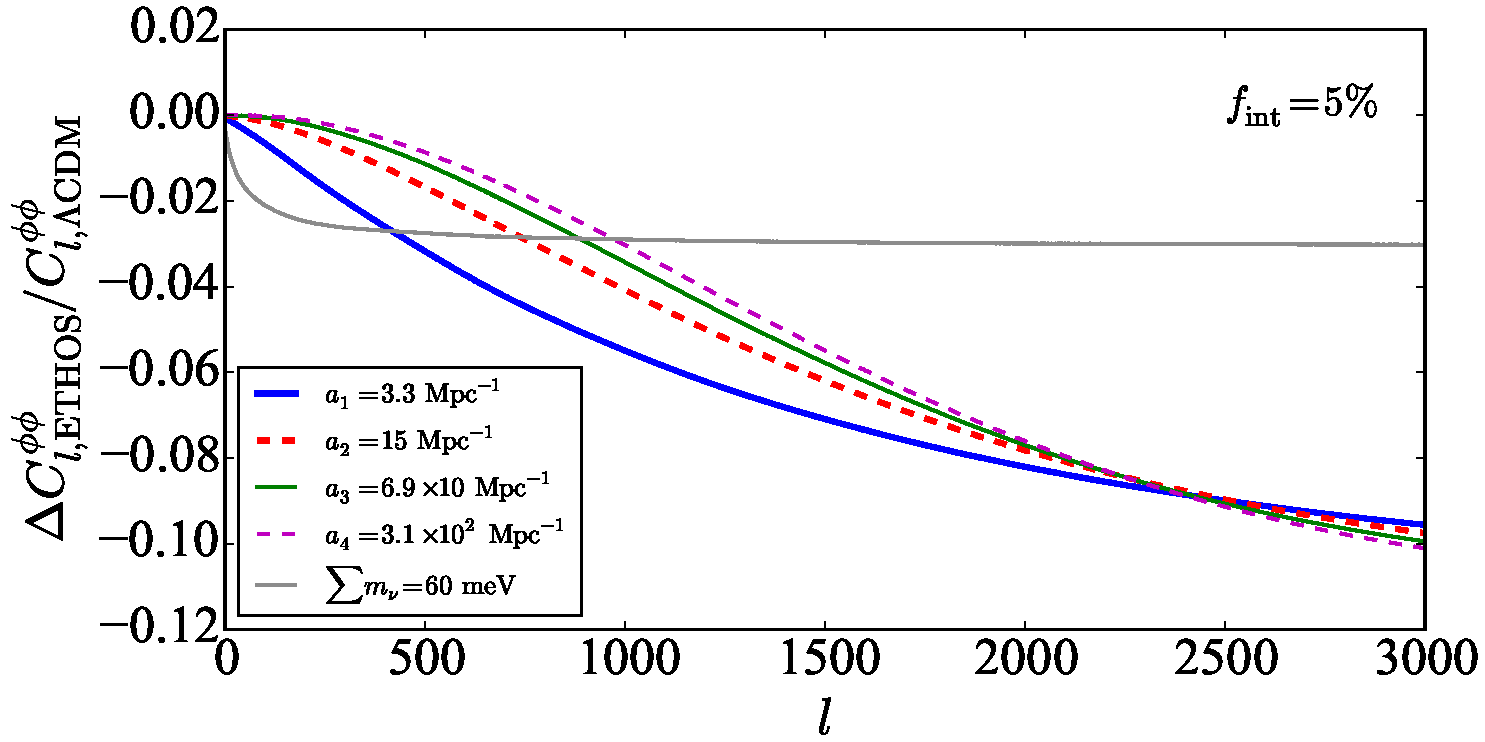
\includegraphics[width=\textwidth]{DarkEnergy/ClsPP_ETHOS_a_n.pdf}\\
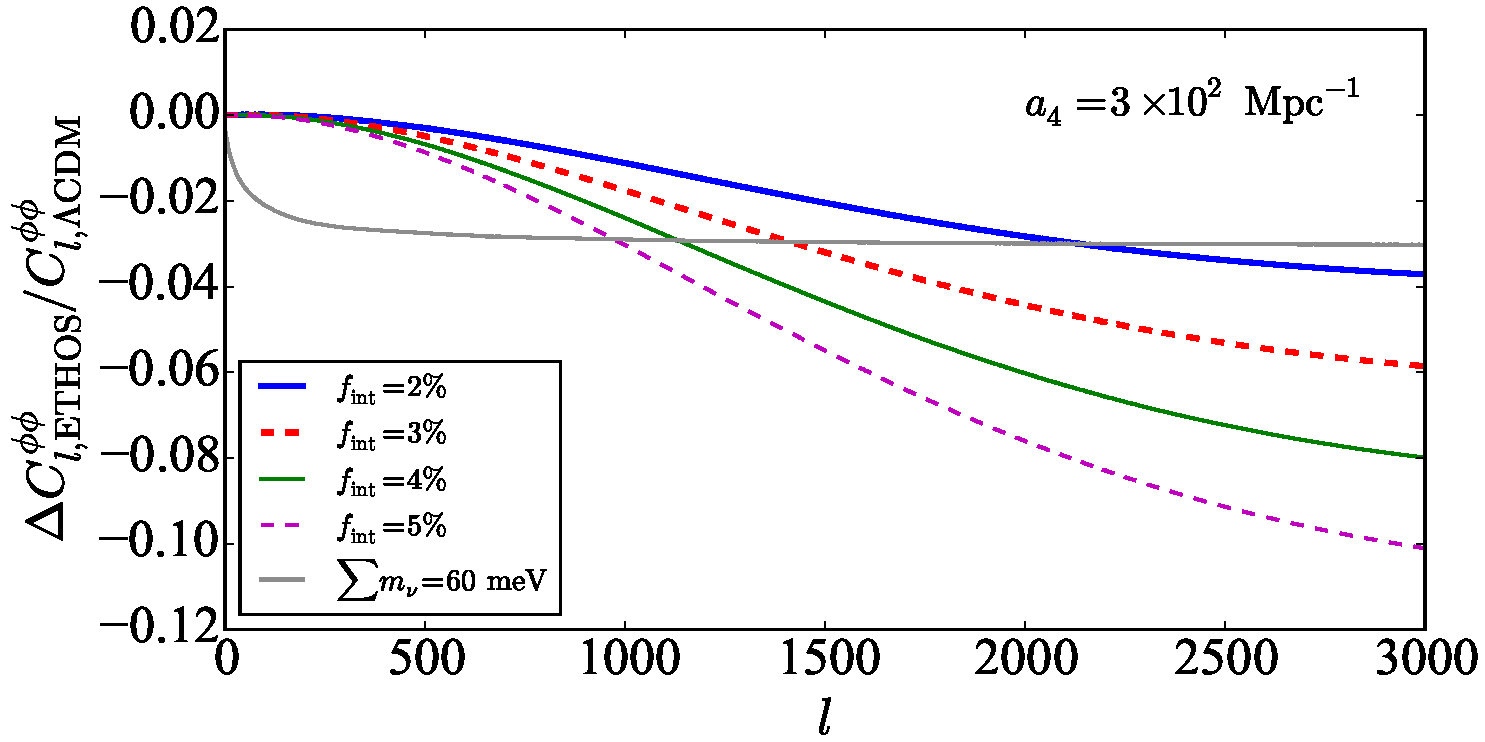
\includegraphics[width=\textwidth]{DarkEnergy/ClsPP_ETHOS_f_int.pdf}
\caption{\emph{Top panel}: Fractional difference of the CMB lensing spectrum between a standard $\Lambda$CDM model (with massless neutrinos) and four different ETHOS models with opacity coefficients $a_n$ given in the legend. In all models shown, $5\%$ of the dark matter is allowed to interact with dark radiation. For comparison, we also display a standard massive neutrino model with $\sum m_\nu =0.06$ meV. \emph{Lower panel}: Similar to the top panel, but we now vary the fraction of dark matter that can interact with dark radiation, for a fixed opacity coefficient of $a_4 = 3\times 10^2$ Mpc$^{-1}$. }\label{fig:Cls_phi_PIDM}
\end{figure}
%

Since non-standard dark matter models affect primarily the large CMB lensing multipoles, the constraining power of CMB-S4 on interacting dark matter is largely independent of the specific choice of $\ell_{\rm min}$. We foresee that the main difficulty in constraining non-standard dark matter theories with CMB-S4 will be the proper modeling of non-linearities in the matter power spectrum, which are quite important for $\ell > 500$. We note that recent progress has been made in this direction \cite{ETHOS2}.


\subsection{Ultralight axions}

Here is the updated text and I've made changes to the .bib file to include those references.

Ultralight axions (ULAs) with masses in the range $10^{-33}~{\rm eV}\leq m_{a}\leq 10^{-20}~{\rm eV}$ are well motivated by string theory, can contribute to either the dark matter or dark energy components of the Universe, depending on their masses, and are distinguishable from DE and CDM in cosmological observables. The current best constraints from the primary CMB TT power, and WiggleZ galaxy redshift survey were made in \cite{hlozek:2015axa}.

The degeneracies of the axions with other cosmological parameters, such as $N_\mathrm{eff}$ or neutrino mass $\sigma$ $m_\nu$ vary depending on the axion mass assumed. Dark energy-like axions with masses around $10^{-33}~{\rm eV}$ change the late-time expansion rate and therefore the sound horizon, changing the location of the acoustic peaks. This has degeneracies with the matter and curvature content.
 Axions that behave more like dark matter (for masses around $m_a \gtrsim 10^{-26}~{\rm eV}$) start oscillating in the radiation era and reduce the angular scale of the diffusion distance, leading to a boost in the higher acoustic peaks, which has a degeneracy with $N_{eff}$.
 In both of these cases, improved errors on the temperature and polarization power spectrum, coupled with constraints on the Hubble constant (for the lightest axions) from Baryon Acoustic Oscillations, lead to improvements in the error on allowed axion energy density of a factor of three.
In the matter power spectrum, and thus CMB lensing power, light axions suppress clustering power, suggesting a degeneracy with effects of massive neutrinos that must be broken to make an unambiguous measurement of neutrino mass using the CMB. The above mentioned effects in the expansion rate likely break this degeneracy.
 
 Adding in information from the lensing reconstruction using S4 will improve constraints on axion DM significantly, and allow one to break the degeneracy between dark-matter like axions and massive neutrinos. A percent-level measurement of the lensing deflection power at multipoles L $>$ 1000 leads to an improvement in the error on the axion energy density of a factor of eight relative to the current Planck constraints, for an axion mass of $m_a=10^{-26}~{\rm eV}$. Furthermore, S4 will improve the maximum axion mass constrainable by the CMB by up to two orders of mangitude from $m_a=10^{-24}~{\rm eV}$ to $m_a=10^{-22}~{\rm eV}$. Achieving this improvement in the mass constraint will require improved understanding of non-linear clustering of axions. If realized it will begin to make contact to the preferred axion model to solve the CDM small scale crises \cite{hu:00a, marsh:2013js}.



%\bibliography{cmbs4}

%%
%% Populate the .bib file with entries from SPIRES Bibtex (preferred)
%% or ADS Bibtex (if no SPIRES entry).
%%  SPIRES will also supply the CITATION line information; please include it.
%%


